%% \listfiles
\documentclass[apj]{emulateapj}
%\documentclass[preprint2,12pt]{emulateapj}
%% \usepackage{natbib}
\usepackage{graphicx}
\usepackage{epsfig}
\usepackage{amssymb,amsmath}
\usepackage{array}
\usepackage{threeparttable}
\usepackage{float}
\usepackage{hyperref}

\singlespace

%definitions
\newcommand{\Msol}{${\rm M_{\sun}}$}

%% Editing markup...
\usepackage{color}


%%%%%%%%%%%%%%%%%%%%%%%%%%%%%%%%%%%%%%%%%%%%%%%%%%%%%%%%%%%%%%%%%%%%%%%%%%%
% WARNING: This LaTeX block was generated automatically by authors.py
% Do not change by hand: your changes will be lost.

%%%%%%%%%%%%%%%%%%%%%%%%%%%%%%%%%%%%%%%%%%%%%%%%%%%%%%%%%%%%%%%%%%%%%%%%%%%

% --------------------- Ancillary information ---------------------
\shortauthors{X.Xu}
\shorttitle{Judy's cta200h project write up}


\begin{document}

\title{Judy's cta200h computing project}
 %% ---------
 
\author{Xiaozheng Xu\altaffilmark{1}}
\altaffiltext{1}{CITA, University of Toronto}

\keywords{pulsars, scintillometry}




\section{Section 1}
\label{sec:1}
\textbf{Question}\textit{: Read and identify giant pulses in the data of the Crab pulsar, taken by the Effelsberg telescope, using the baseband reading package: \url{https://github.com/mhvk/baseband}}



This part is done using a helper script written by Robert GPbaseband.py in EVNcrab in the package scint\_analysis  \url{https://github.com/ramain/scint_analysis}. 

\section{Section 2}
\label{sec:2}
\textbf{Question}:\textit{: Coherently de-disperse a giant pulse. Plot the dynamic spectrum of the dispersed pulse, the de-dispersed pulse, and determine the Signal/Noise (S/N) of the pulse summed over all frequencies.}


Originally, the data of a giant pulse is a 1D array consisting of the $2^{22}$ electric field strength values measured by the telescope through time. These time values are then grouped into $2^{22}/(2*256) = 8192$ time bins. The values in each of the 8192 time bins is then fourrier transformed into 256 frequency values (because all values are real, a rfft is used, so the number of frequencies is half of the number of time values). These frequency values are than plotted against their time bins as a frequency vs time matrix. This matrix is the dynamic spectrum. 

The sampling rate of the telescope is 32MHz. The value of each time bin is 2*256/32MHz = 16$\mu$s. Accordingly, I converted the units of time from 0-8192 to the actual time values. There are 16 threads of data, and 2 direction of polarization, resulting in 8 total threads. These 8 threads correspond to increasing frequency bands, which can be seen as the 8 horizontal bands in Fig. \ref{fig:dedispersed} and Fig. \ref{fig:dispersed}. Each thread spans a frequency value of 16 MHz, based on the frequency valeus from the fourrier transform. The base observation is 1610.49 MHz, which is used to get a range for the frequency axis. 

Originally, the giant pulse consisting of different frequencies get emitted from the pulsar at the same time. The Interstellar Medium (ISM) disperses the pulse, causing lower frequencies to arrive later than higher frequencies.\cite{coherent dedispersion} To revert this effect, the coherent dedispersion method is used (as implemented in Robert's code). 

The largest giant pulse in all30.txt is in scan15 2015-10-19T01:23:57.220212, with a S/N of 90. Thus, I chose to plot the spectres and S/N for this pulse. Fig. \ref{fig:dedispersed} plots the de-dispersed dynamic spectrum, Fig. \ref{fig:dispersed} plots the dispersed dynamic spectrum, and Fig. \ref{fig:SN} shows the signal to noise of the de-dispersed pulse.

\begin{figure}[H]
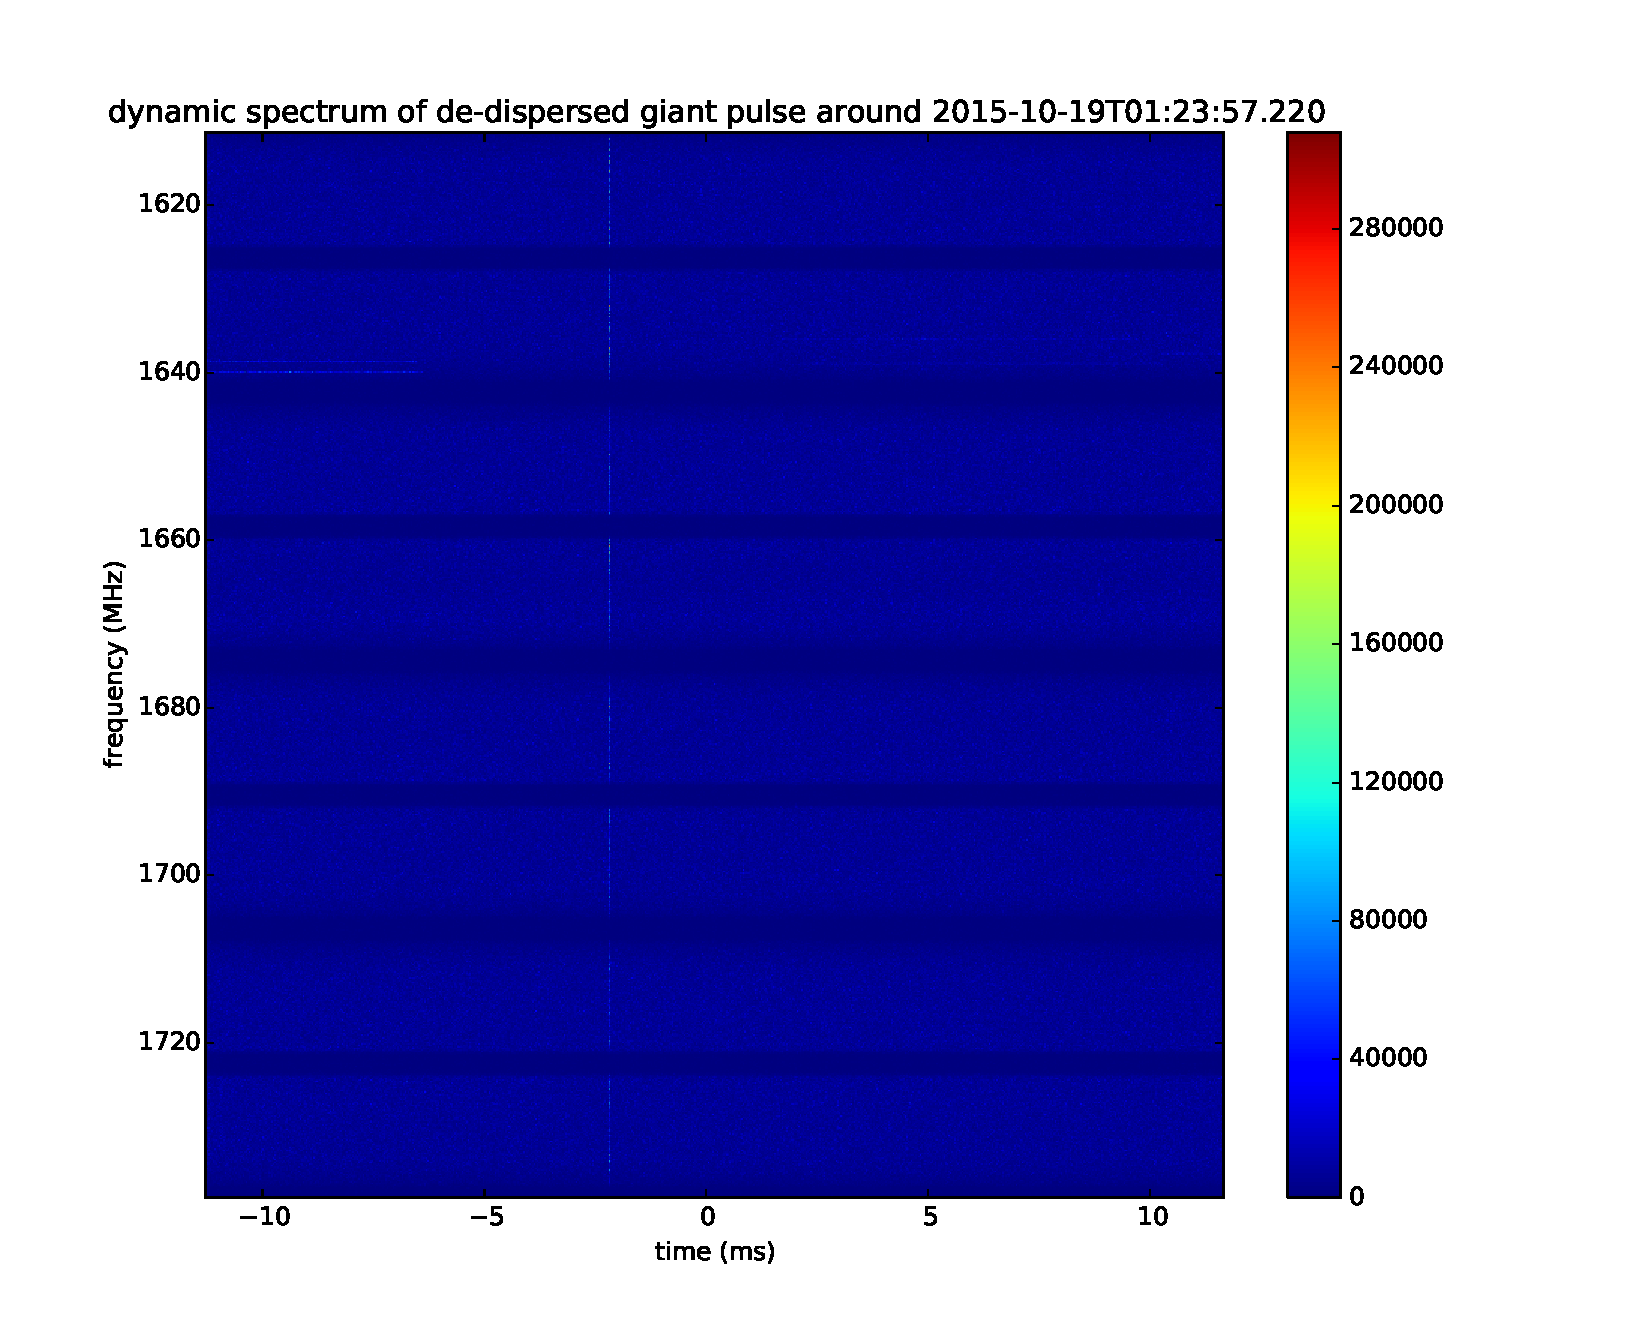
\includegraphics[width=1.0\columnwidth]{dedispersed_spec.pdf}
\caption{The dynamic spectrum of the de-dispersed pulse}
\label{fig:dedispersed}
\end{figure}

\begin{figure}[H]
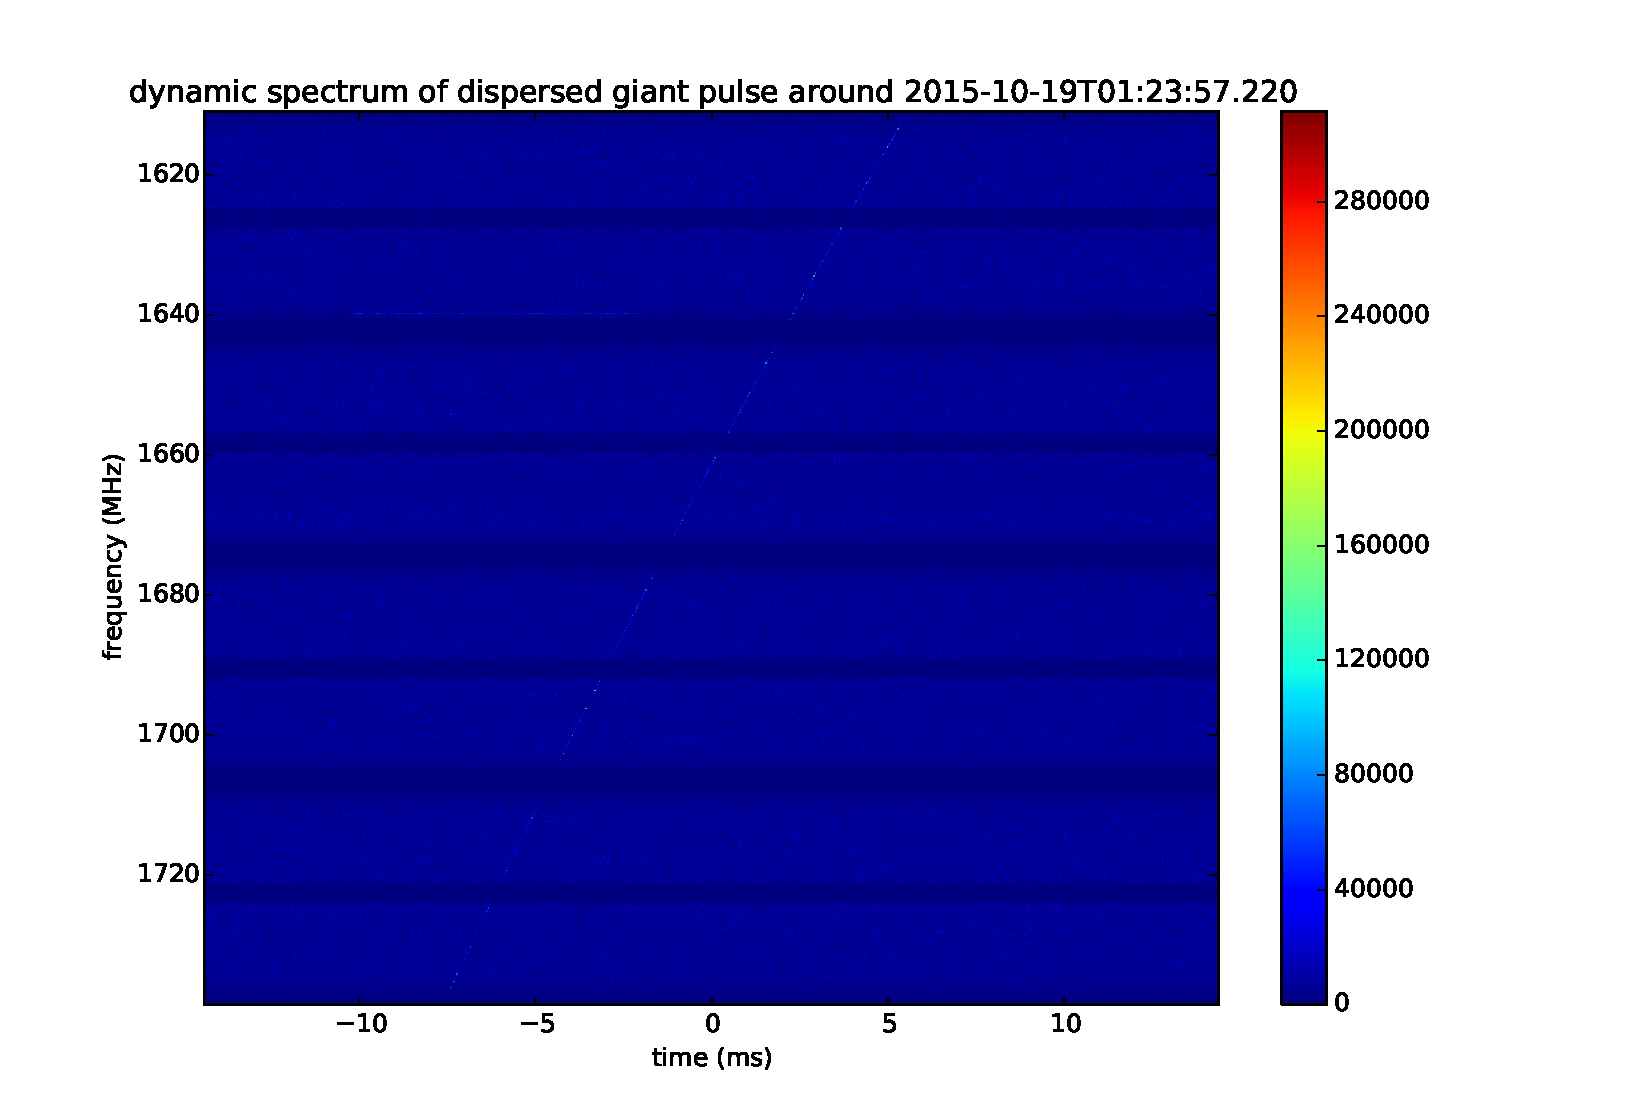
\includegraphics[width=1.0\columnwidth]{dispersed_spec.pdf}
\caption{The dynamic spectrum of the dispersed pulse. The Interstellar Medium (ISM) disperses the pulse, causing lower frequencies to arrive later than higher frequencies.\cite{coherent dedispersion}}
\label{fig:dispersed}
\end{figure}

The signal to noise of the pulse is calculated using the de-dispersed dynamic spectrum as in Eq. \ref{eq:SN}. First, sum all the frequencies over each time bin to get a 8192 long 1D array $D$. Then, find the mean $m$ and standard deviation $\sigma$ of the noise from the first 1000 elements of this array (the pulse usually occur near the center-somewhere between 3900 and 4200). Subtract the whole array from $m$ and divide by $\sigma$. The S/N of the pulse is the max in the matrix.     

\begin{equation}\label{eq:SN}
    S/N(t) = \frac{D(t)-m}{\sigma}
\end{equation}


\begin{figure}[H]
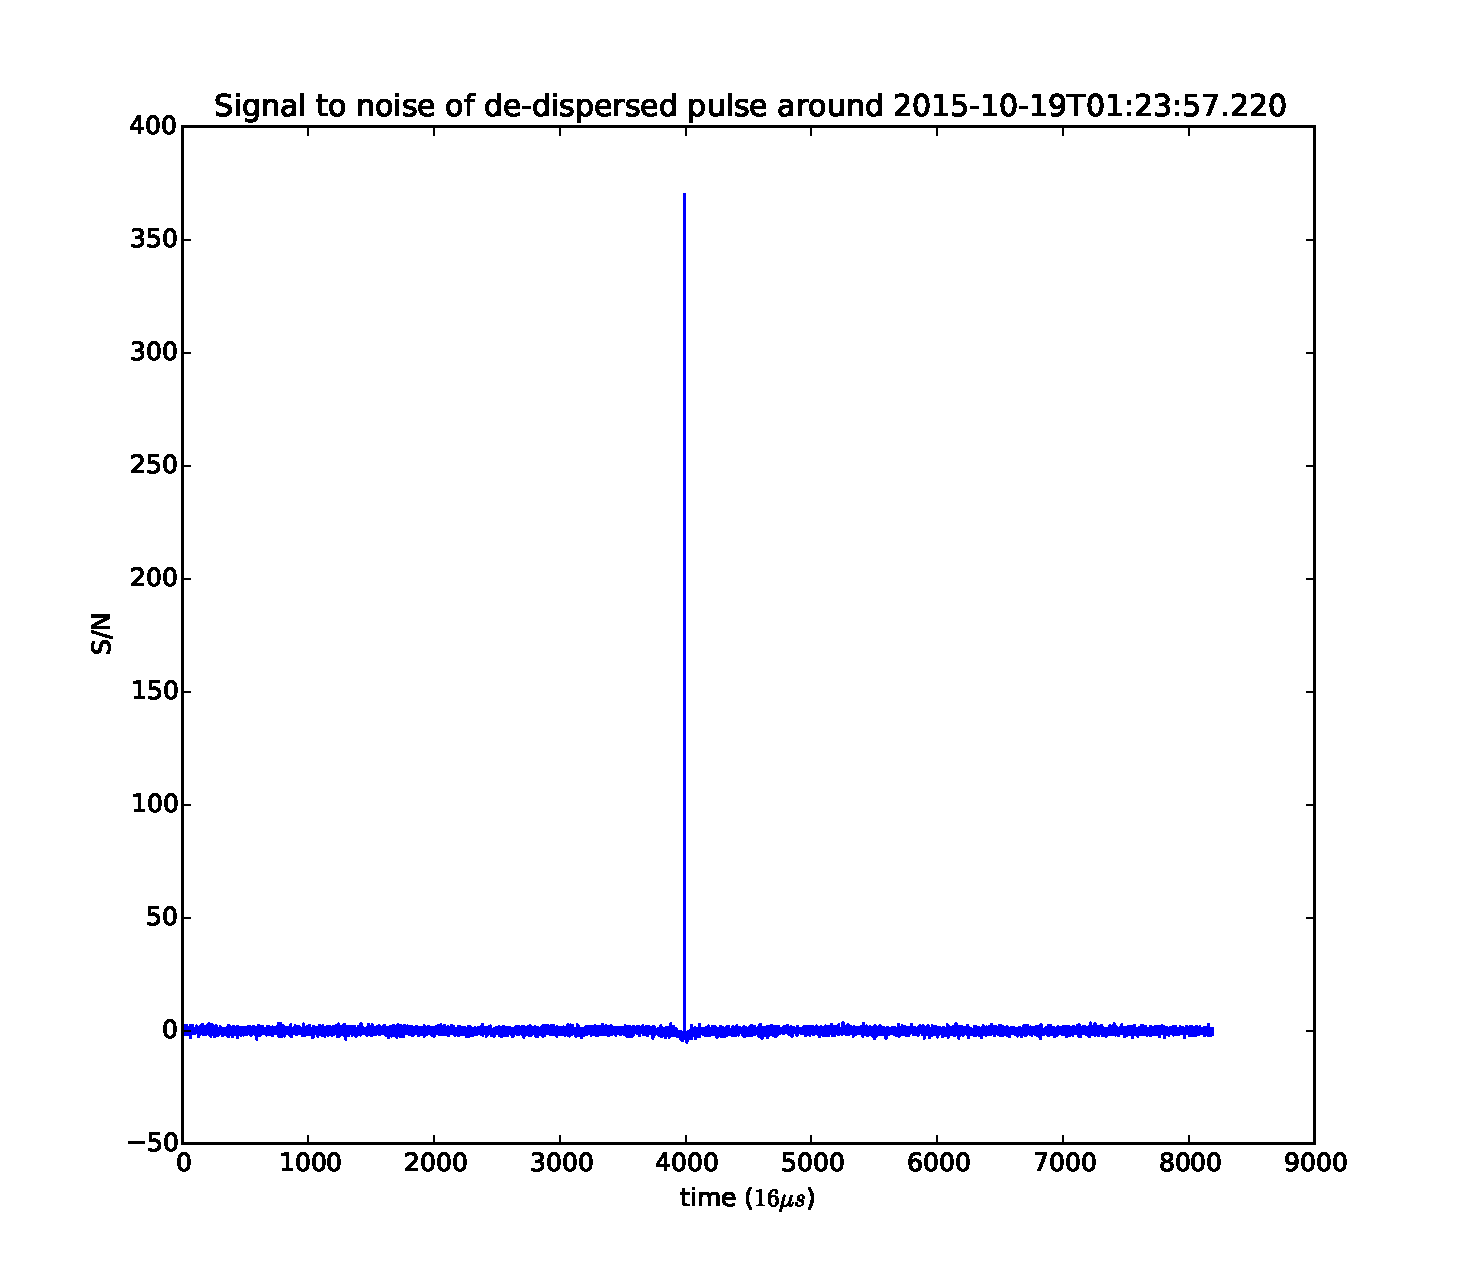
\includegraphics[width=1.0\columnwidth]{S-N.pdf}
\caption{Signals to noise of the de-dispersed pulse. The pulse has a S/N of around 370 summed over all 8 frequency bands.}
\label{fig:SN}
\end{figure}


\section{Section 3}
\label{sec:3}
\textbf{Question}\textit{: Compare the frequency spectrum of at least two giant pulses and calculate a measure of the correlation between them. Time permitting, compute the correlation coefficient of all pulse pairs as a function of time separation between them (this is a larger scale goal, and realistically will take a couple of weeks).}

The frequency spectrum can be taken directly from the frequency values corresponding to the pulse time in the de-dispersed spectrum. Fig. \ref{fig:figureOfSpectrum} shows that for the 8 frequency bands.

\begin{figure}[H]
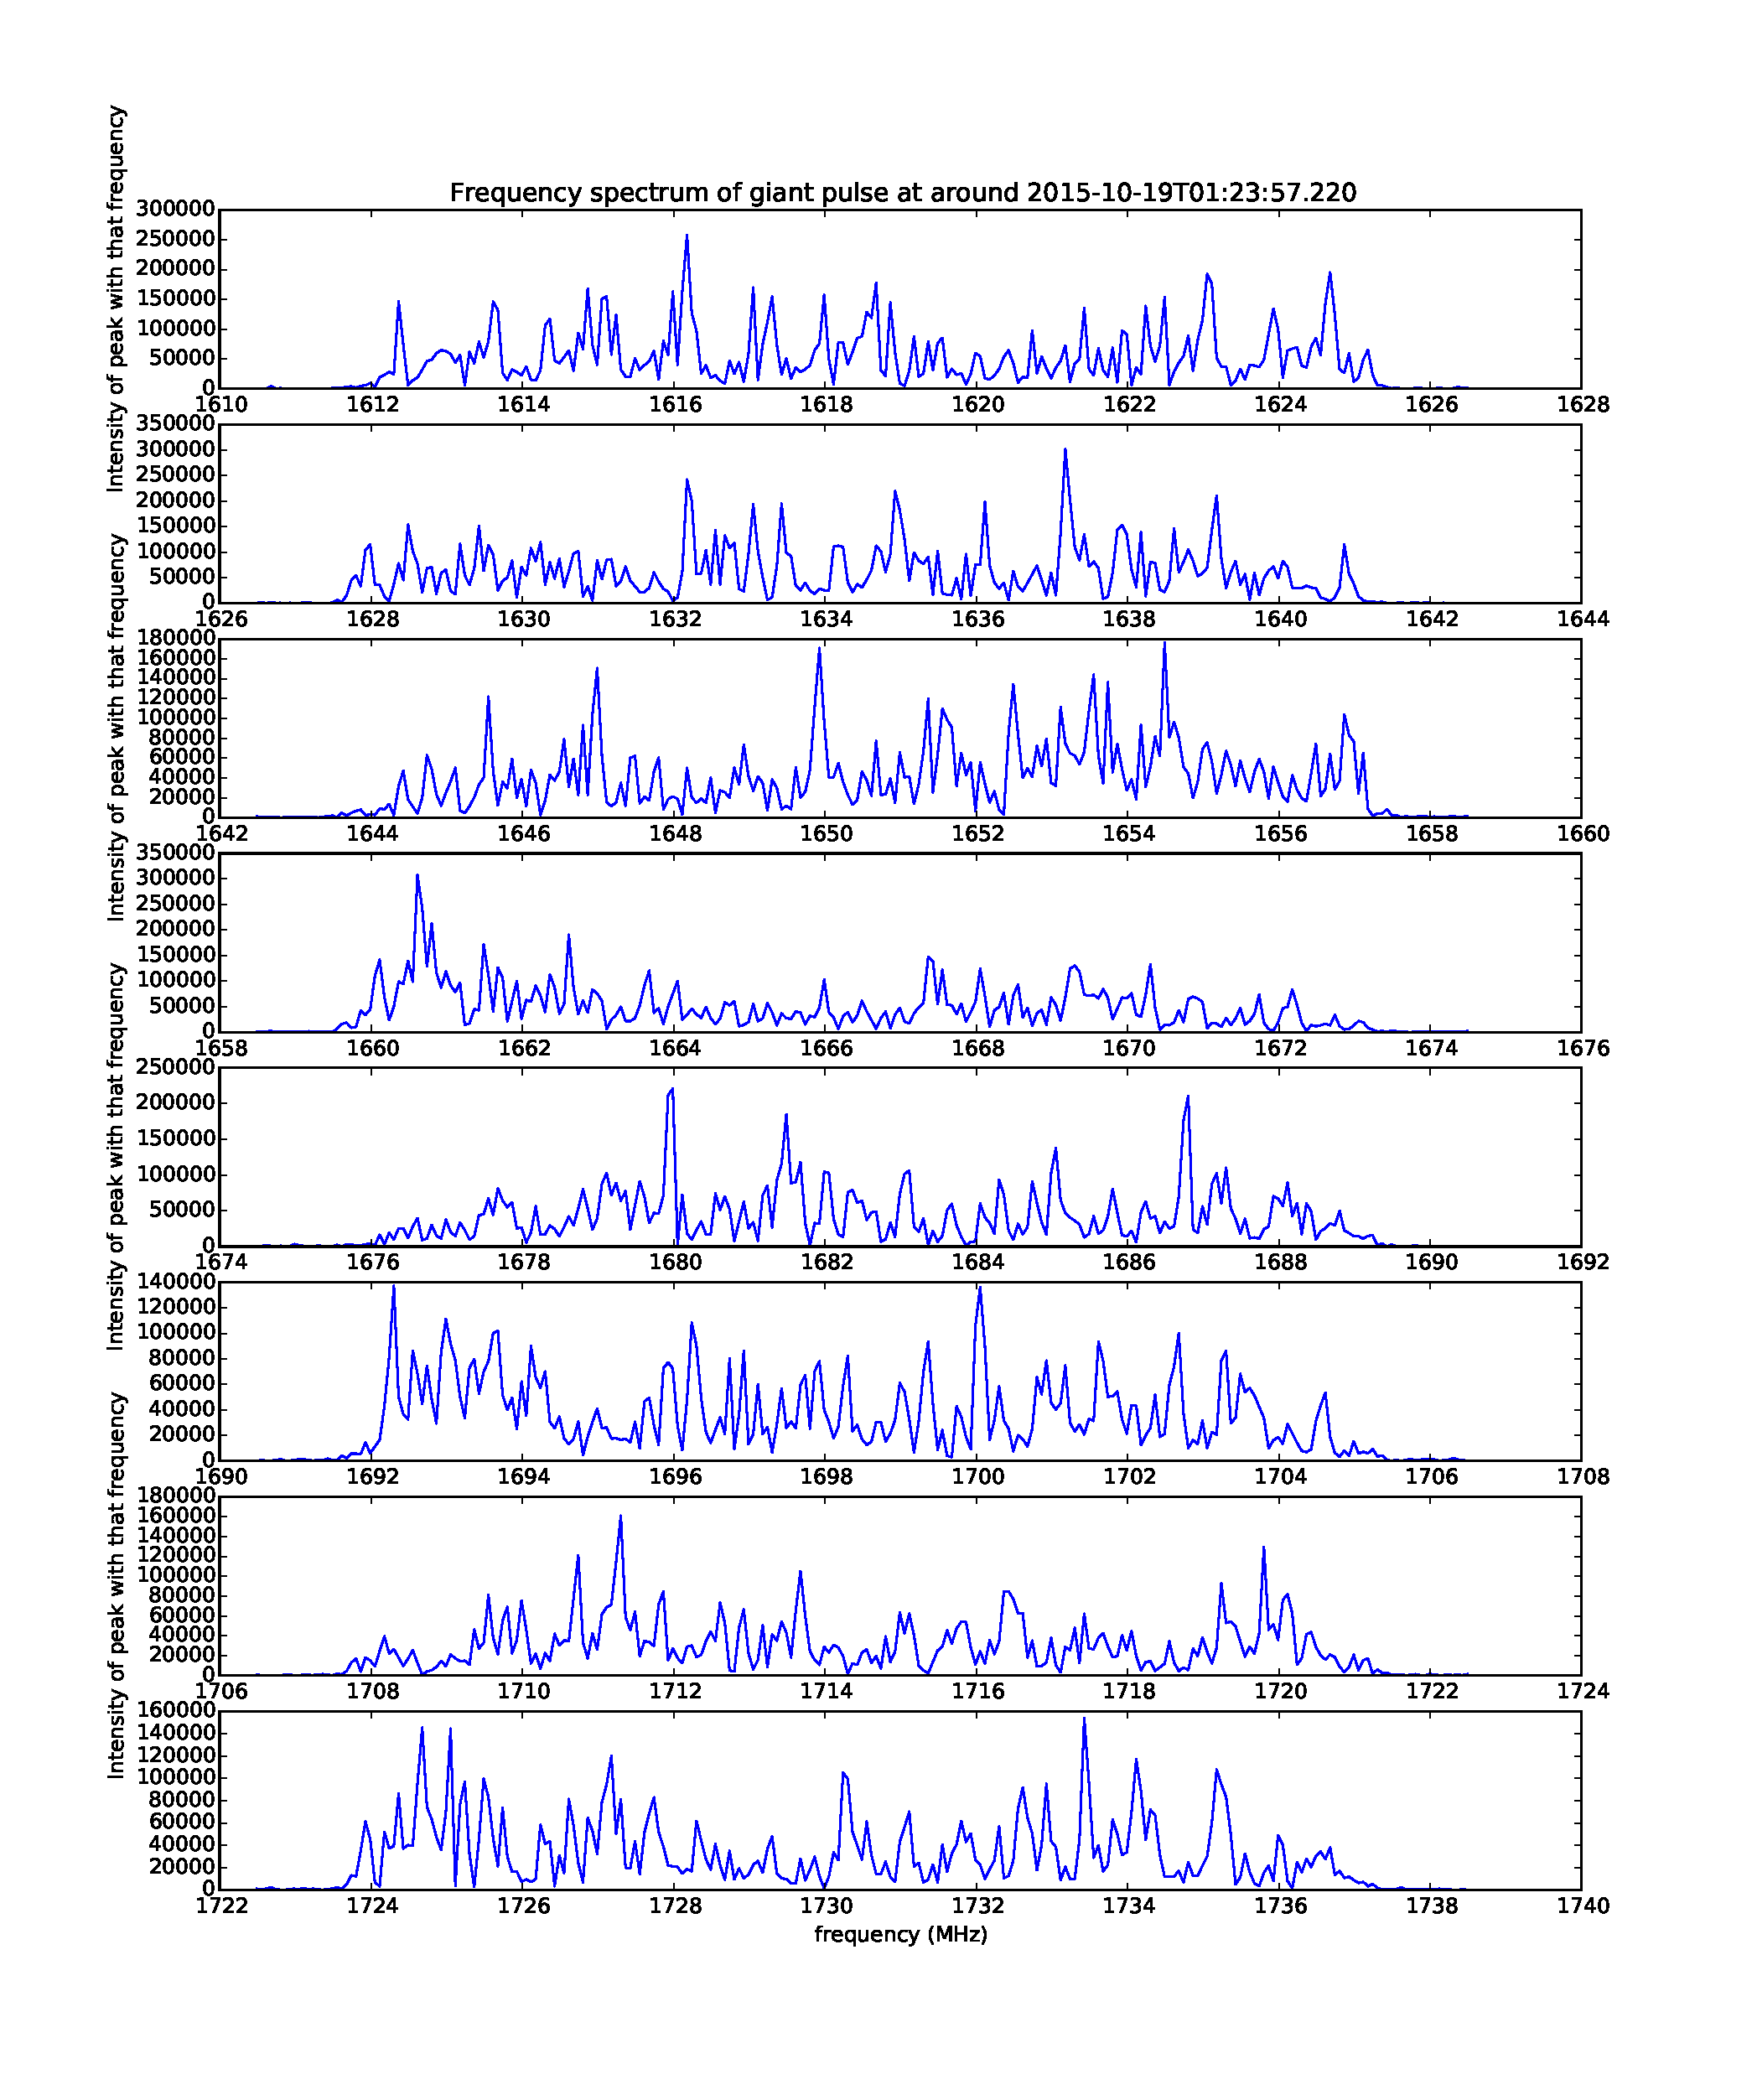
\includegraphics[width=0.9\columnwidth]{all30_1_freq_spec.pdf}
\caption{Frequency spectrum of the giant pulse mentioned in Section \ref{sec:2}}
\label{fig:figureOfSpectrum}
\end{figure}

A correlation coefficient of the frequency spectre of two giant pulses is found using np.corrcoef. Fig. \ref{fig:freq_spec2} and Fig. \ref{fig:freq_spec2_1} shows the frequency spectre of two pulses plotted together, their correlation coefficient and their corresponding time lag.

\begin{figure}[H]
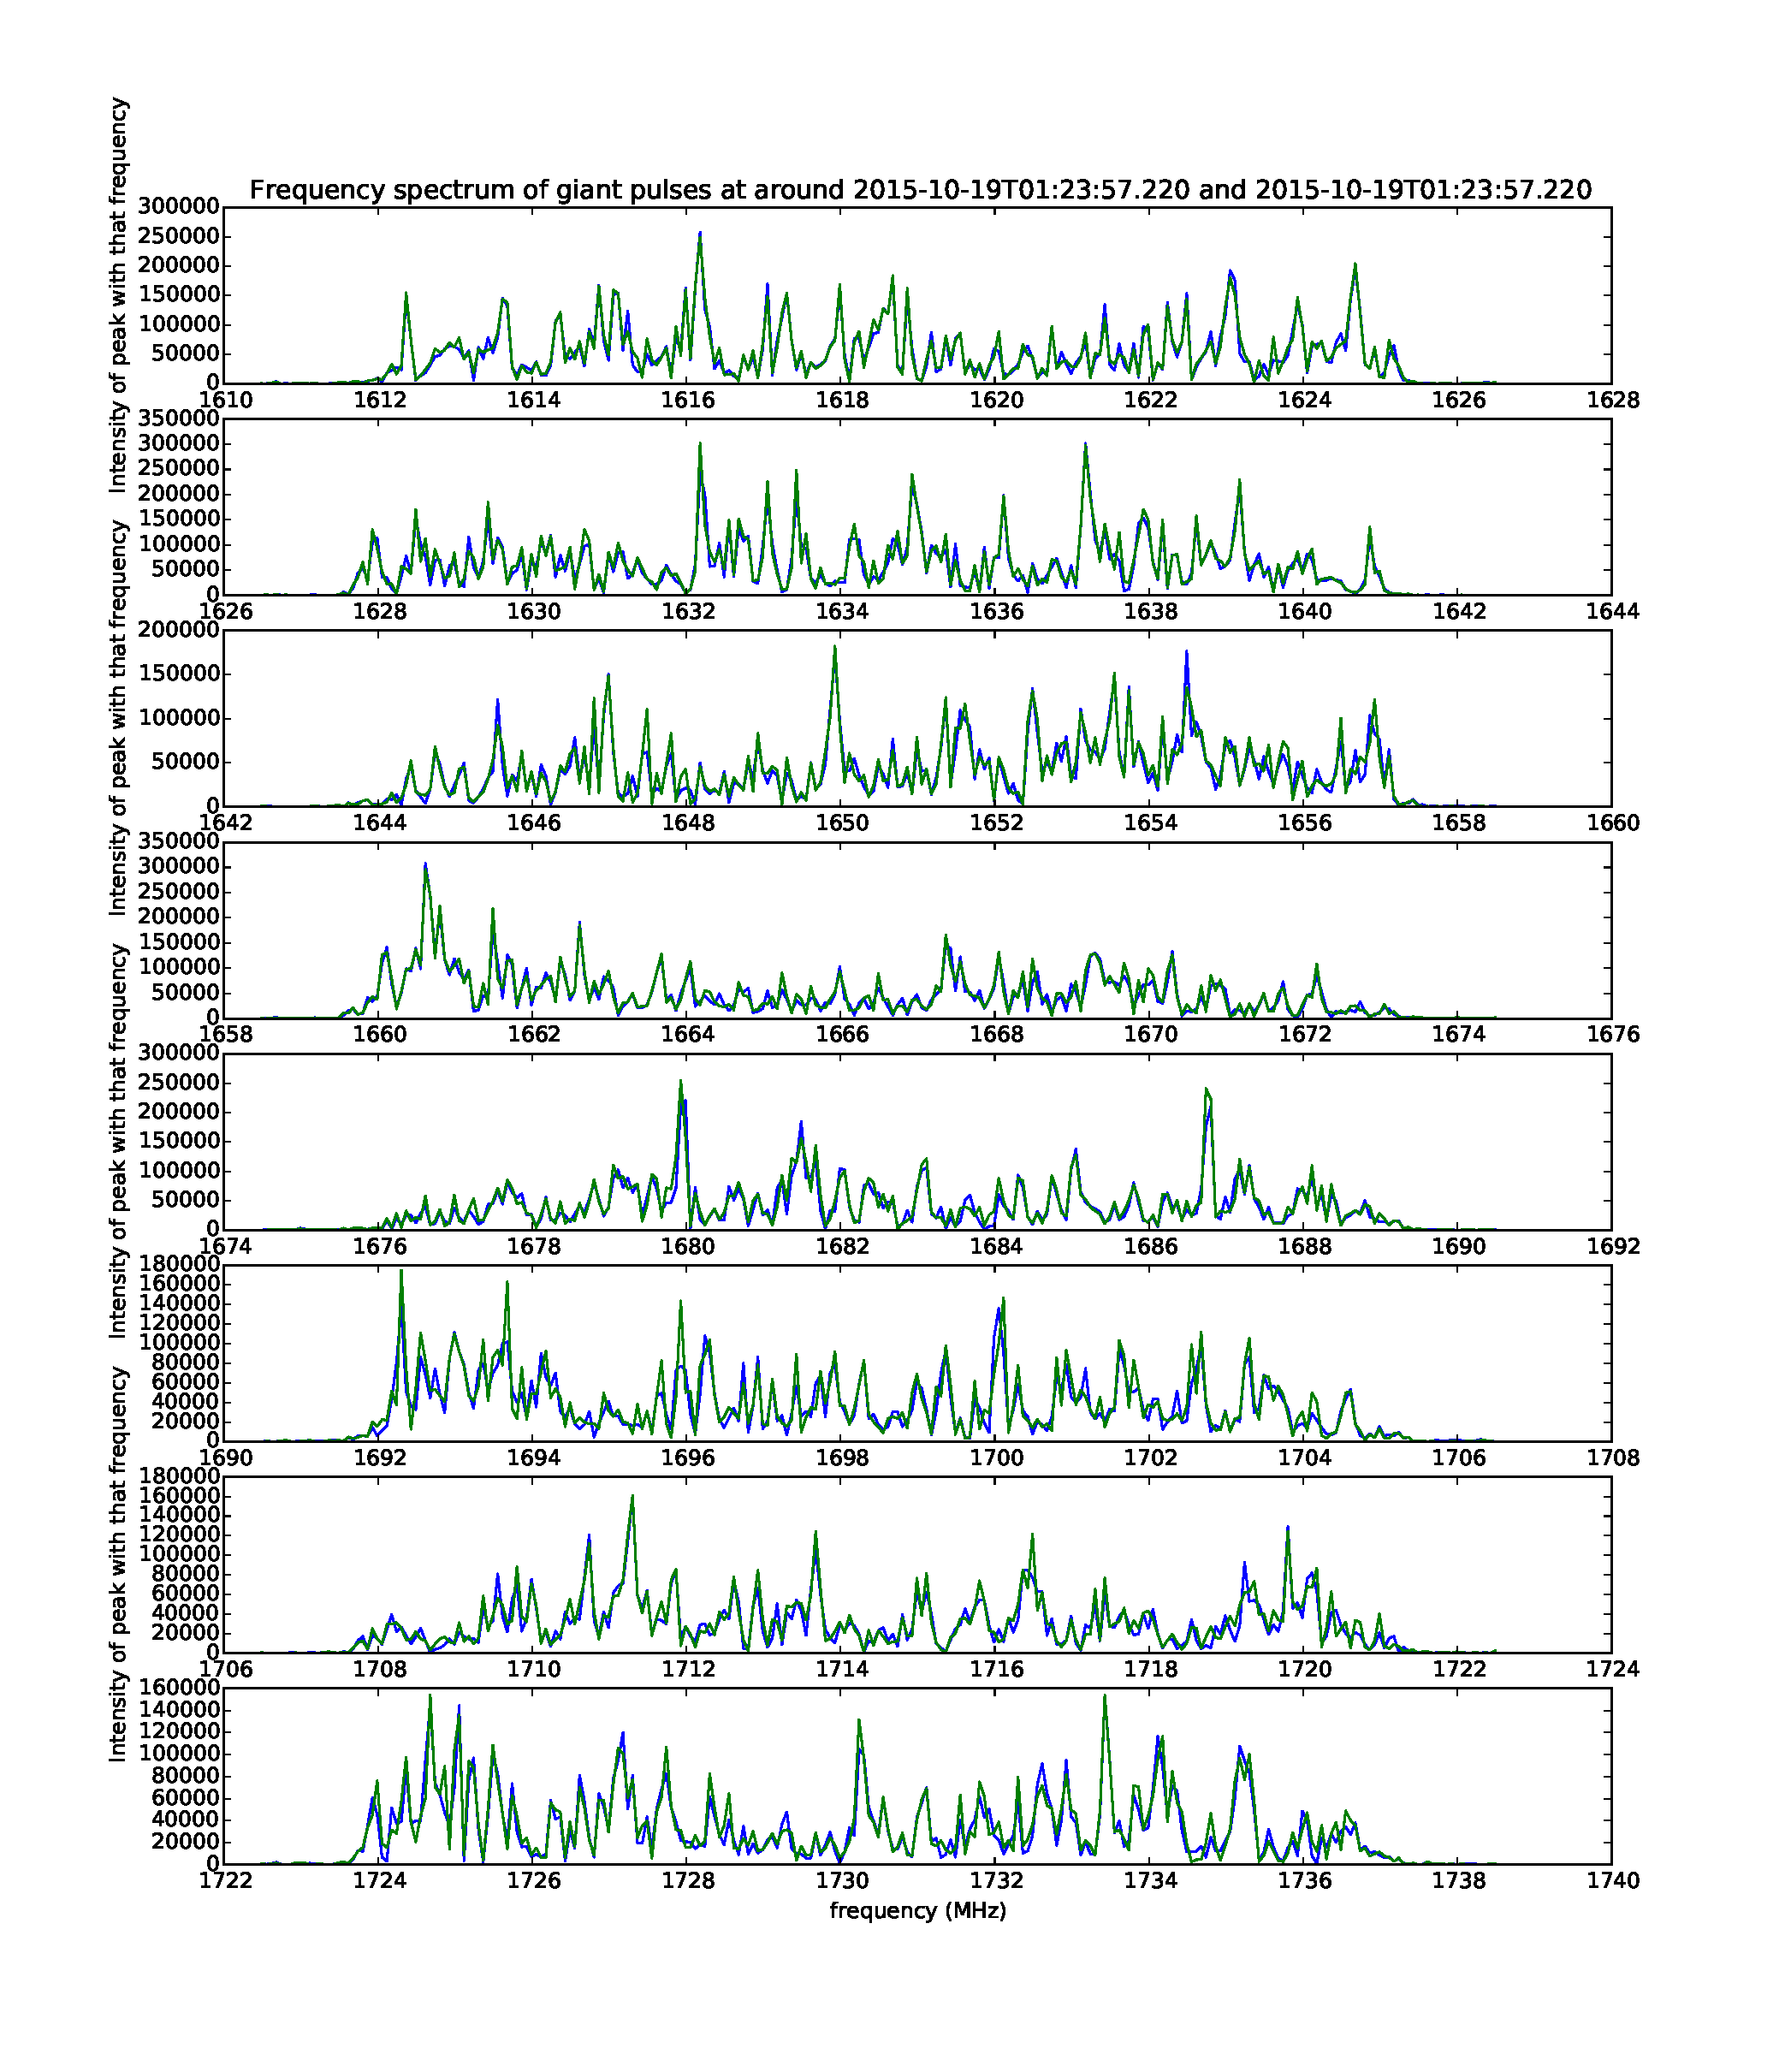
\includegraphics[width=0.9\columnwidth]{co_freq_spec_2mus.pdf}
\caption{The two pulses has a correlation coefficient of 0.937, and has a time lag of 2$\mu$s}
\label{fig:freq_spec2}
\end{figure}

\begin{figure}[H]
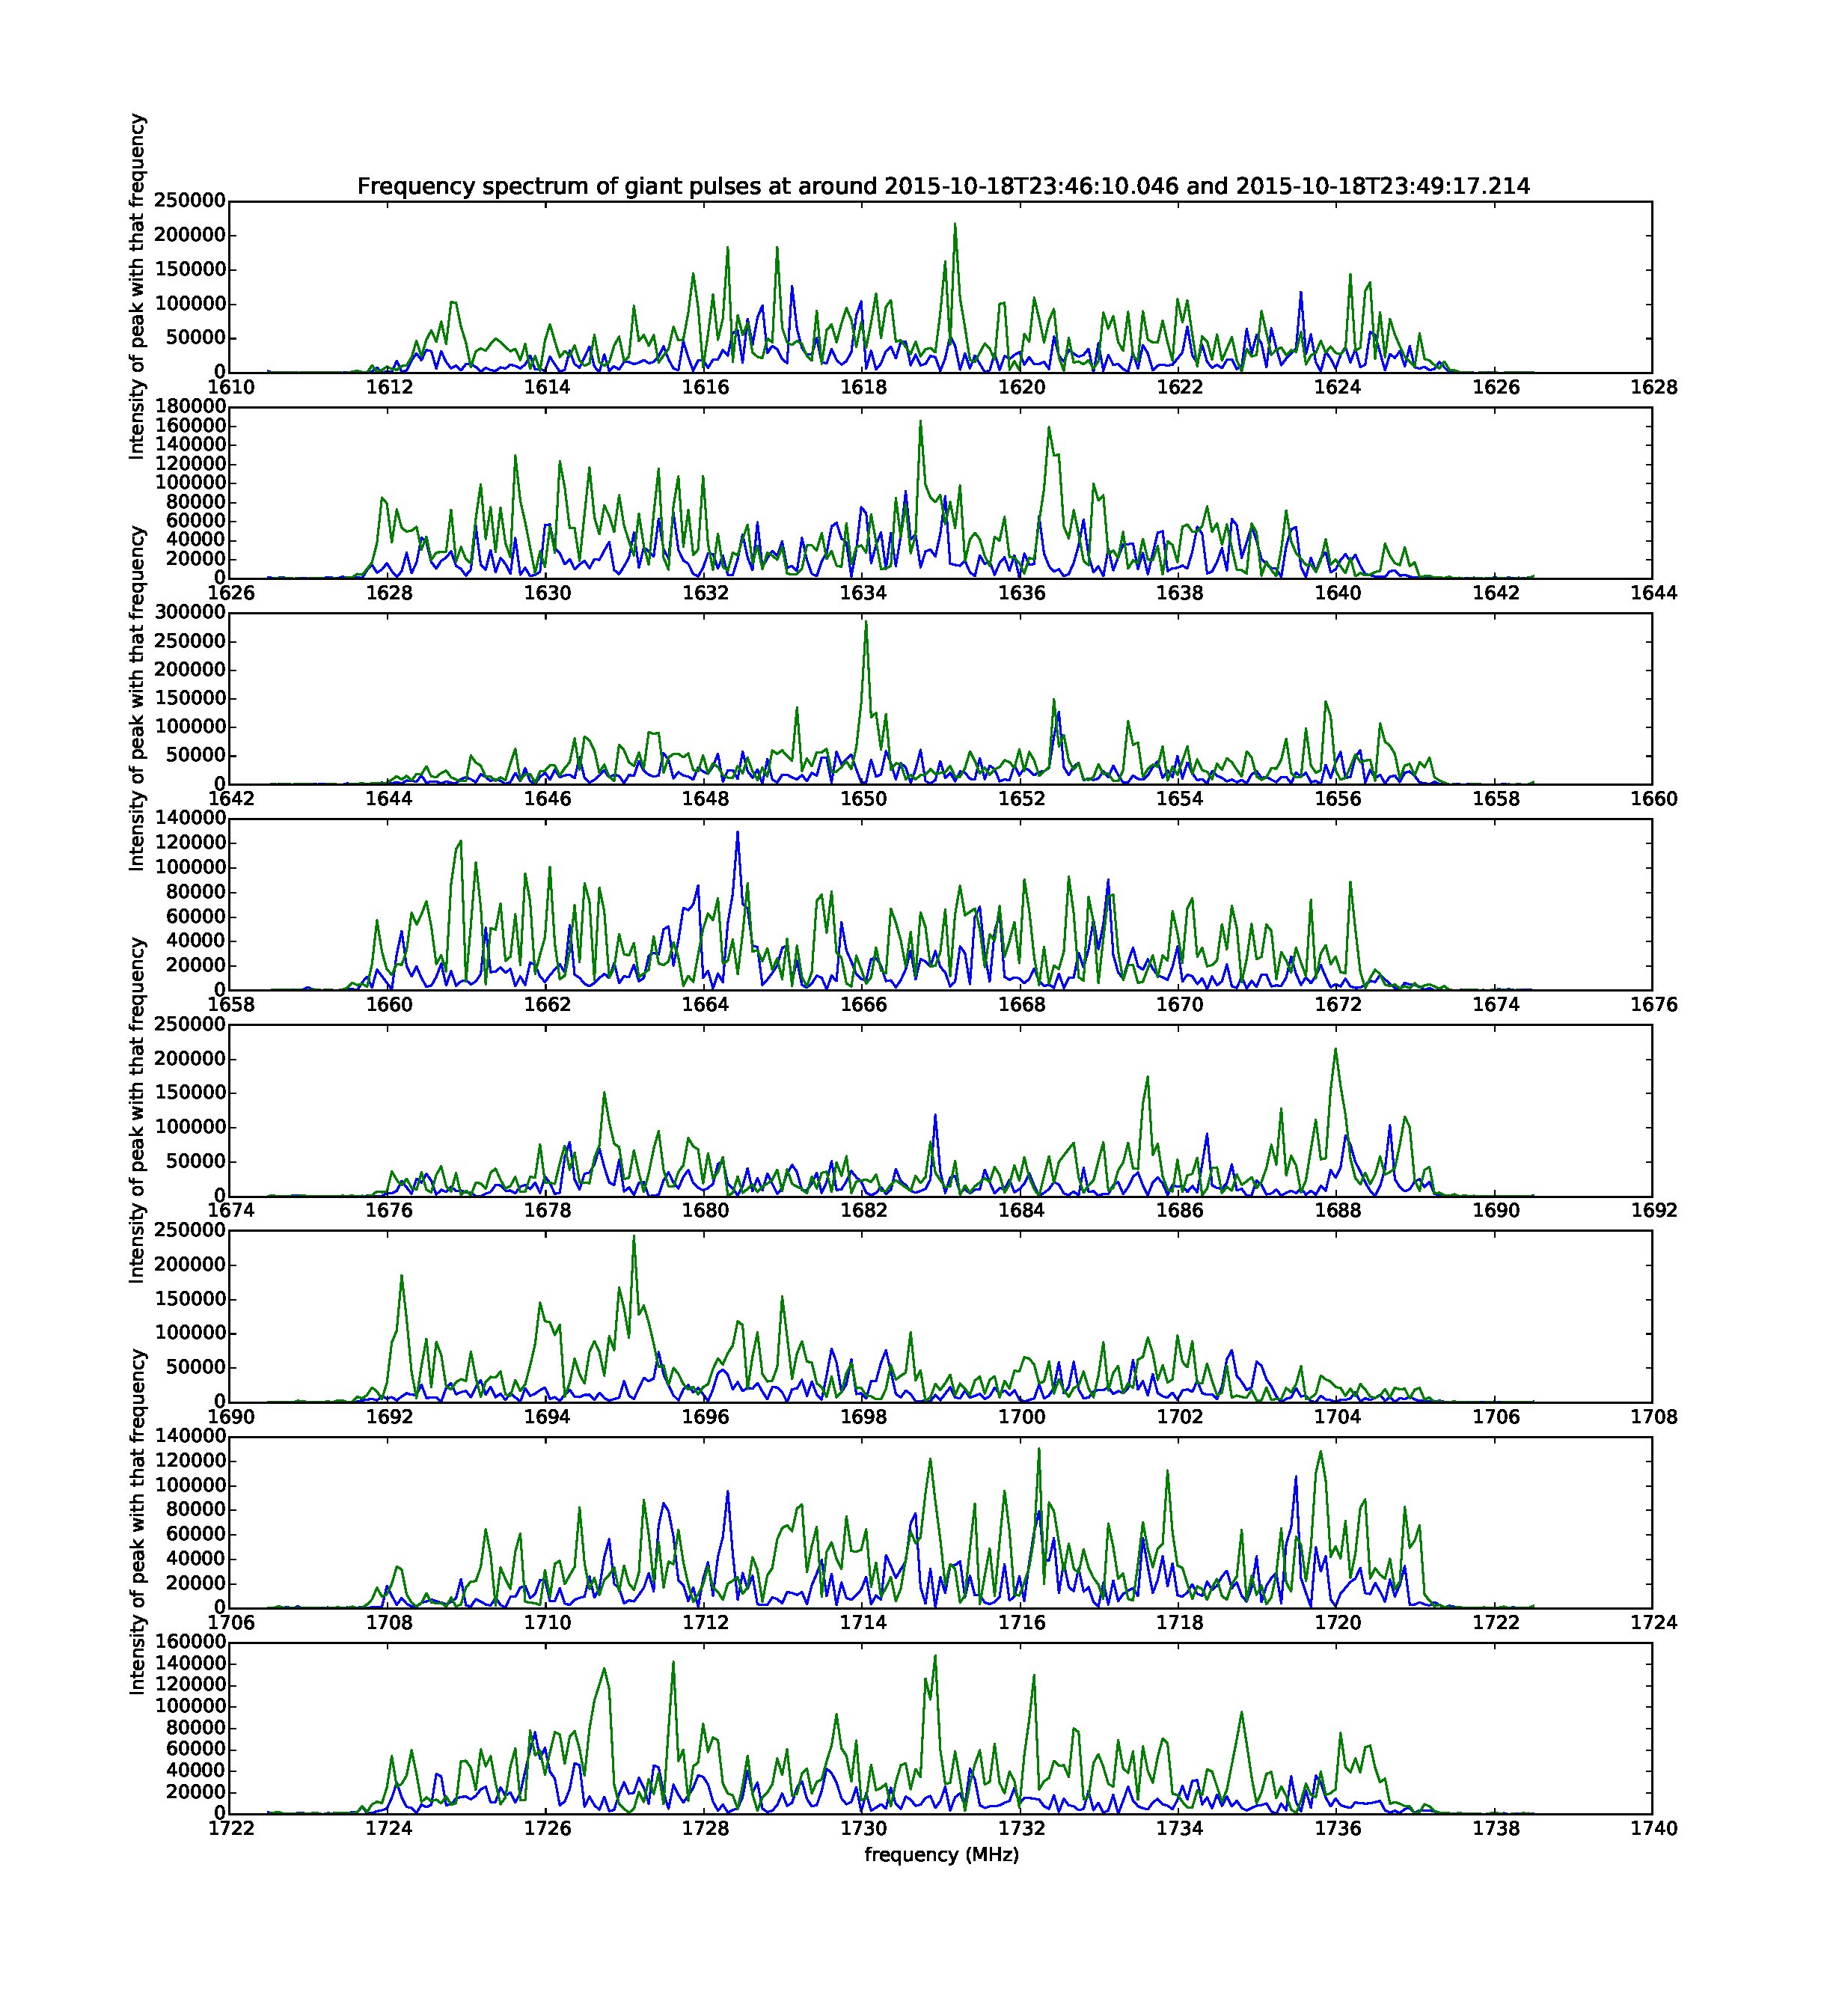
\includegraphics[width=0.9\columnwidth]{co_freq_spec_2mus1.pdf}
\caption{The two pulses has a correlation coefficient of 0.108, and has a time lag of 187.16s}
\label{fig:freq_spec2_1}
\end{figure}

The correlation coefficients are found for many pulse pairs. I did this by looping through the pulses in all30.txt, all20.txt and all10.txt, while varying the index difference between the two pulses. A plot of the correlation coefficients vs time lag is shown in Fig. \ref{fig:coeffs}. For time lag on the order of 10e-6, the correlation coefficients are high and they decrease as time lag increases. For time lag on the order of seconds, the correlation coefficients are between 0 and 0.2, and distributed quite randomly.


\begin{figure}[H]
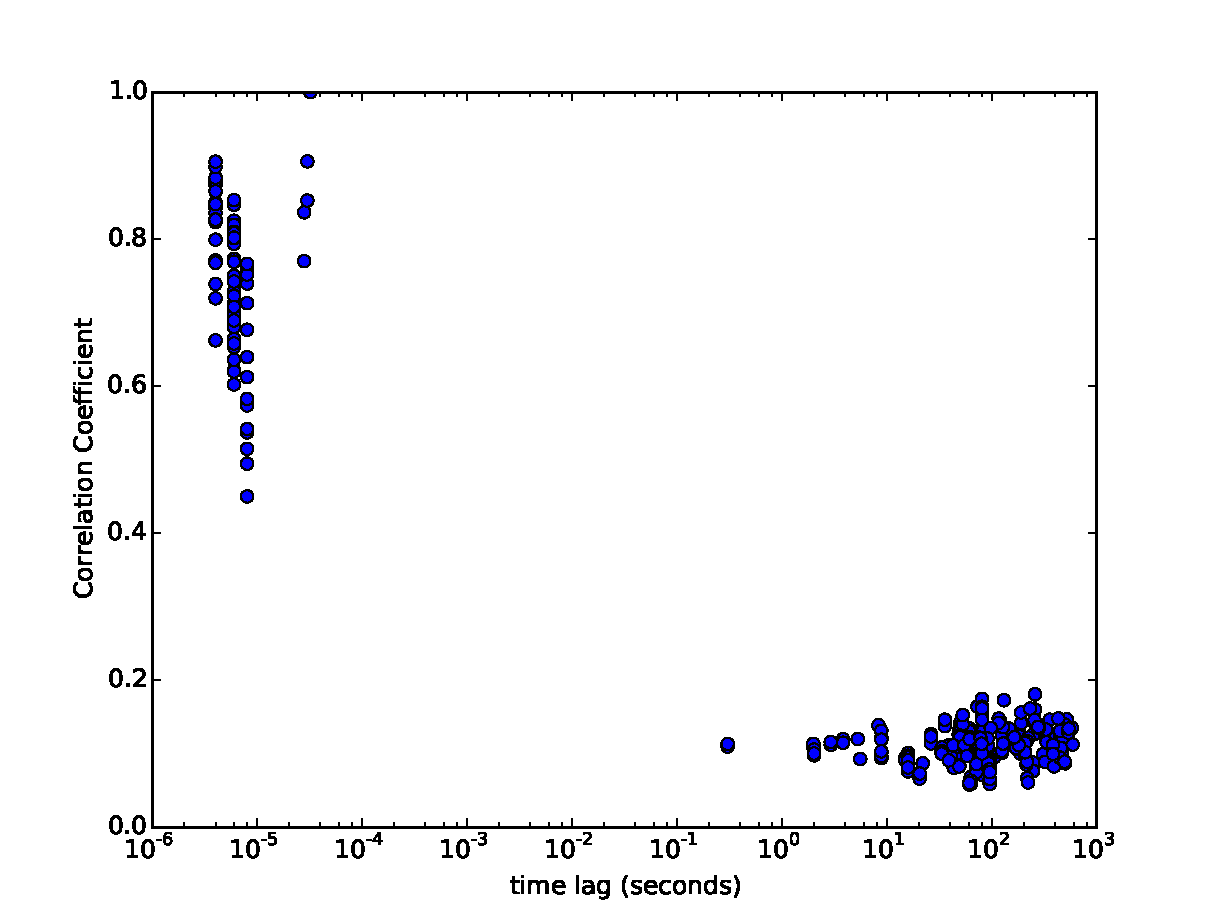
\includegraphics[width=1.0\columnwidth]{May12_coeff.pdf}
\caption{A plot of the correlation frequency vs time lag between 2 giant pulses. There are about 160 data points in total.}
\label{fig:coeffs}
\end{figure}


% \begin{table}[H]
% \begin{center}
% \begin{threeparttable}
% \caption{A table.}
% \begin{tabular}{|l|c|c|}
% \hline 
% Col 1 & Col 2 & Col 3 \\
%  \hline  
% Val 1 & Val 2 & Val 3 \\
% Val 1 & Val 2 & Val 3 \\
% \hline
% \end{tabular} 
% \vskip 2mm
% \begin{tablenotes} \item  
% \begin{center}
% \begin{flushleft}
% Description of table.
% \end{flushleft}
% \end{center}
% \end{tablenotes}
% \label{tab:vitalStats_kappa}
% \end{threeparttable}
% \end{center}
% \end{table}


%\acknowledgments



\begin{thebibliography}{lenscib_refs.bib,apj-jour}
\bibitem{coherent dedispersion}
Pulsar Observations II. -- Coherent Dedispersion Polarimetry, and Timing.
Stairs, I. H. 2002ASPC..278..251S
\end{thebibliography}


\end{document}
